\documentclass[a4paper]{article}
\usepackage{graphicx} % Required for inserting images
\usepackage[margin = 2.8cm]{geometry} 
\usepackage{palatino}
\usepackage{listings}
\usepackage{xcolor}
\usepackage{hyperref}

\lstdefinestyle{mypython}{
  language=Python,
  basicstyle=\ttfamily\footnotesize,
  keywordstyle=\color{green}\bfseries,
  stringstyle=\color{blue},
  commentstyle=\color{gray}\ttfamily\itshape,
  showstringspaces=false,
  breaklines=true
}

\lstset{style=mypython}

\title{ELEC0447 -- Project 1 \\ Low voltage distribution feeder modeling and analysis}
\author{Bertrand Corn\'elusse, Geoffrey Bailly}
\date{October 2, 2025, version 1.0}

\begin{document}

\maketitle

\begin{center}
    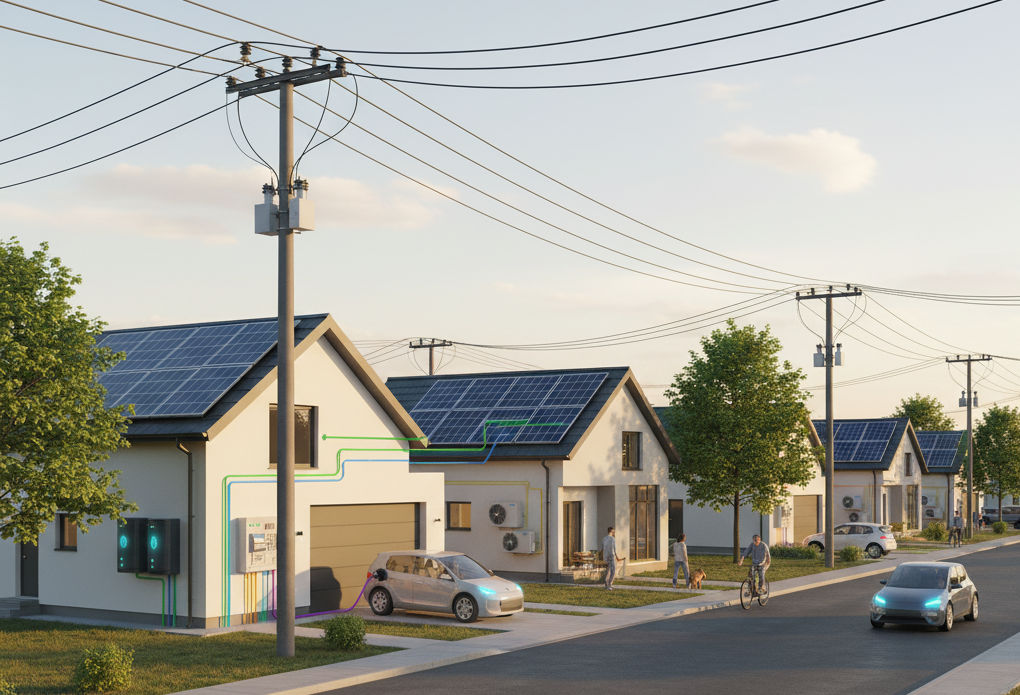
\includegraphics[width=0.99\linewidth]{Gemini_Generated_Image_djxmz2djxmz2djxm.png}
    Image generated by Google Gemini (what's wrong with this picture?) 
\end{center}

\section{Introduction}
The goals of this assignment are to
\begin{enumerate}
    \item get familiar with Python and PandaPower, a power system modeling tool
    \item learn to run some first power-flow analyses on a simple network
    \item gain some intuition on the impact of high loads and renewable distributed generation
    \item compare three-phase balanced and unbalanced operating conditions.
\end{enumerate}

Let's consider a street where two distribution network feeders connect ten houses. A \textit{feeder} is a power line that carries electricity from a substation or distribution transformer, which we will model as our slack bus, to the end-users. 
The network data is provided as an Excel file with separate sheets that describe the buses, lines, and loads.

\begin{center}
\textit{Remark: we used PandaPower version 3.1.2 to carry out all the experiments below.}   
\end{center}

\newpage

\section{Your tasks}
\begin{enumerate}
\item \textbf{(Base case)} Write a Python code to model a \textbf{single-phase equivalent }of the network and run a first power flow analysis\footnote{An example code for a 3-bus network is available as a link in the slides on the power flow analysis. You can use it as a starting point. You should also consult PandaPower's documentation.}.
\item Explore the results of the base case. Plot the network schematic and the voltage magnitude and angle evolution along the feeders. Display the line loading coefficients. Briefly discuss the results.
\item Starting from the base case, progressively increase the load (keep the same power factor) at the buses near the end of the feeder (this simulates the addition of electric vehicles or heat pumps). What do you observe? Is there a loading condition such that the power flow does not converge? Explain.
\item Starting from the base case, add photovoltaic plants at the buses near the end of the feeders and progressively increase their production (from 1 to 10kW). What do you observe? 
\item \textbf{(3-phase base case)} Now, you will model the network more accurately using a model of the three phases. Update the model to run a three-phase power flow. 
\begin{enumerate}
\item First, update the cable type to encode the \textit{zero-sequence parameters}\footnote{This is to model the coupling between the phases. You must not fully understand what is done here, browse the internet if you want to know more.} of the line
\begin{lstlisting}[language=Python, caption=Updating the cable type.]
import pandapower as pp
pp.create_std_type(net, {"r_ohm_per_km": 0.642, "x_ohm_per_km": 0.083,
                "c_nf_per_km": 210., "max_i_ka": 0.142,
                "endtemp_degree": 70.0, "r0_ohm_per_km": 1.923,
                "x0_ohm_per_km": 0.249,
                "c0_nf_per_km":  70}, name="unsymmetric_NAYY 4x50 SE",element = "line")
line_type = "unsymmetric_NAYY 4x50 SE" # To be used when creating the lines.
\end{lstlisting}
and then use this line type to create the lines.
\item Using the function \lstinline{pp.create_asymmetric_load}, load the system so that you are \textbf{in the same conditions than in the base case }(with the \textbf{single-phase equivalent }). Use star (or wye) connected loads.
\item Add the following commands to run the power flow\footnote{Again, no need to understand everything, it is required to make it work.}:
\begin{lstlisting}[language=Python, caption=Running a three-phase power flow analysis.]
net.ext_grid['s_sc_max_mva'] = 1000
net.ext_grid['rx_max'] = 0.1
pp.add_zero_impedance_parameters(net)
pp.pf.runpp_3ph.runpp_3ph(net, algorithm='nr', calculate_voltage_angles=True)
\end{lstlisting}
\item If it succeeds, you can now access the results in the \lstinline|net| object (e.g. \lstinline{net.res_bus_3ph.vm_a_pu}).
\end{enumerate}
\item Explore the results of the 3-phase base case. Plot the evolution of the magnitudes and angles of the voltage along the feeder (from bus 0 to bus 10). Display the currents in the phases and the neutral along the feeder. Briefly discuss the results.
\item Starting from the 3-phase base case, load the network so that the total load at each bus is equally shared between phase a and phase b. What can you observe?
\item Start from the 3-phase base case. By chance, all homeowners connected a 2 kVA photovoltaic inverter on phase a. Model this situation when the inverters all produce the maximum active power. What do you observe? What could you do to improve the situation? Note: a photovoltaic inverter is indivisible.
\item Simulate the situation where 
\begin{enumerate}
    \item a 3-phase fault cuts the line between the transformer and the first bus of the first feeder; 
    \item The line connecting the ends of the two feeders is activated.
\end{enumerate}
Repeat the last analysis with the inverters on phase a.
\end{enumerate}

\section{Submission rules} 
\begin{enumerate}
    \item Work by groups of 2.
    \item Submit on Ecampus
    \begin{itemize}
        \item a report in PDF format with an average of half a page per question
        \item your Python notebook (a zip if multiple files).
    \end{itemize} 
    \item Do nice, readable, and interpretable plots $\rightarrow$ \href{https://www.youtube.com/watch?v=rUV8VFbUi_U}{Tutorial video}.
    \item Due date: November 4, 2025, 23:59.
\end{enumerate}



\end{document}
